\begin{figure}[H]
	\centering
	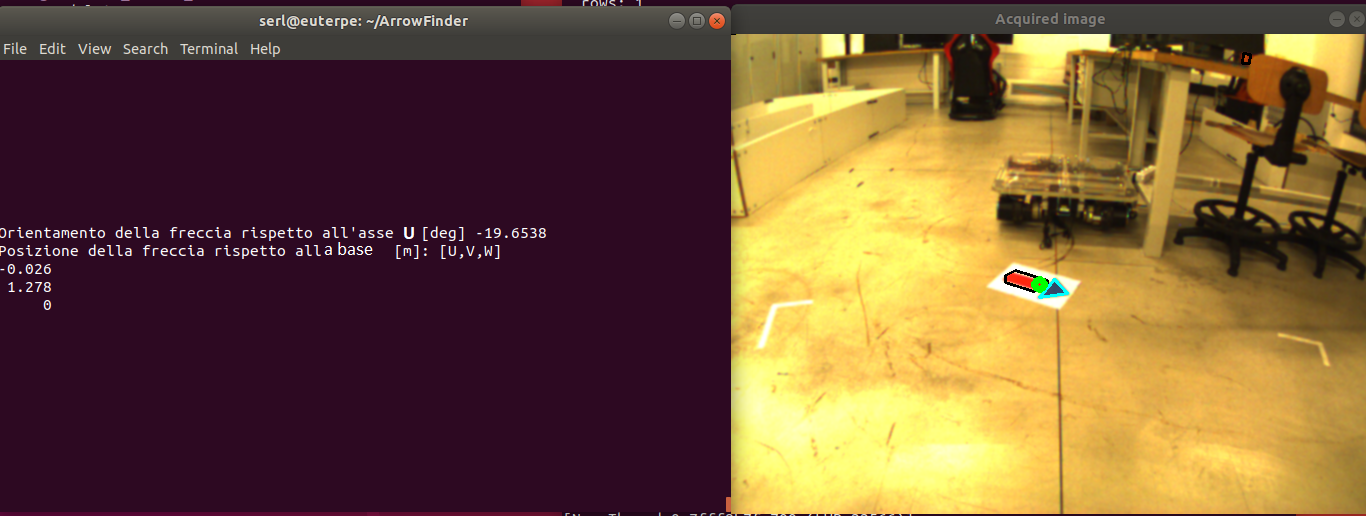
\includegraphics[width=0.8\textwidth]{Immagini/FinalResult.png}
	\caption{Esempio esplicativo del risultato finale dell'algoritmo}
	\label{fig:finalResult}
\end{figure}

Ciò che si legge in Fig.\ref{fig:finalResult} è l'output visivo che si è deciso di realizzare:
esso rappresenta la posizione e l'angolo $\Theta$ della freccia più grande che l'algoritmo è riuscito ad identificare nell'immagine acquisita.

Da notare che è possibile identificare le frecce senza avviare l'algoritmo di calcolo della posizione nelle world coordinates: in questo modo l'algoritmo di riconoscimento delle frecce può essere usato per trovare frecce appese ai muri o alle pareti. 